\documentclass{article}

\usepackage[a4paper, left=1.5cm, right=1.5cm, top=2cm, bottom=2cm]{geometry}
\usepackage{../../../components/components}
\usepackage{fancyhdr}
\usepackage{tikz}
\usepackage{hyperref}

% Configuration des en-têtes et pieds de page
\pagestyle{fancy}
\fancyhf{} 

\fancyhead[L]{Préparation CAPES}
\fancyhead[C]{Géométrie}
\fancyhead[R]{2025 - 2026}

\fancyfoot[L]{Ewen Rodrigues de Oliveira}
\fancyfoot[R]{\thepage}

\begin{document}

\docTitle{Géométrie plane et dans l'espace}

\noindent Ce document propose une synthèse (rapide et probablement non exhaustive) des notions de géométrie plane et dans l'espace abordées au collège, avec des démonstrations détaillées des théorèmes fondamentaux.

\section{Bases de la géométrie plane et configurations élémentaires}

\subsection{Éléments fondamentaux et vocabulaire}

\definition{Soient deux points distincts $A$ et $B$. 
\begin{itemize}
    \item La \textbf{droite} $(AB)$ est l'ensemble infini des points alignés avec $A$ et $B$.
    \item Le \textbf{segment} $[AB]$ est la portion de droite délimitée par les points $A$ et $B$. Sa longueur est notée $AB$.
    \item La \textbf{demi-droite} $[AB)$ est la portion de droite commençant au point $A$ (l'origine) et passant par $B$.
    \item Le \textbf{milieu} d'un segment $[AB]$ est le point $I$ de ce segment tel que $AI = IB$.
\end{itemize}
}

\vocabulary{Pour traduire l'appartenance d'un point à une droite, on utilise le symbole $\in$. Si trois points appartiennent à une même droite, on dit qu'ils sont \textbf{alignés}.}

\subsection{Relations géométriques}

\definition{Deux droites sont dites \textbf{perpendiculaires} si elles se coupent en formant un angle droit. Deux droites sont dites \textbf{parallèles} si elles ne se coupent jamais ou si elles sont confondues.}

\theorem{Propriétés des droites}{Parallélisme et perpendicularité}{true}{
\begin{itemize}
    \item Si deux droites sont parallèles à une même troisième droite, alors elles sont parallèles entre elles.
    \item Si deux droites sont perpendiculaires à une même troisième droite, alors elles sont parallèles entre elles.
    \item Si deux droites sont parallèles, toute droite perpendiculaire à l'une est perpendiculaire à l'autre.
\end{itemize}
}

\begin{center}
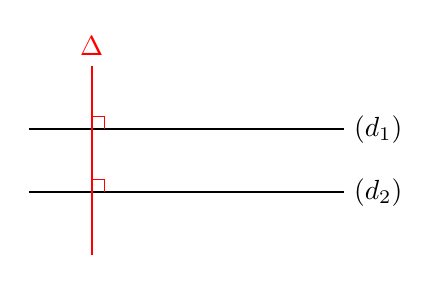
\begin{tikzpicture}[scale=0.8]
    \draw[thick] (0,1) -- (5,1) node[right] {$(d_1)$};
    \draw[thick] (0,0) -- (5,0) node[right] {$(d_2)$};
    \draw[thick, red] (1,-1) -- (1,2) node[above] {$\Delta$};
    \draw[red] (1,1) ++(0.2,0) -- ++(0,0.2) -- ++(-0.2,0);
    \draw[red] (1,0) ++(0.2,0) -- ++(0,0.2) -- ++(-0.2,0);
\end{tikzpicture}
\captionof{figure}{Si $(d_1) \parallel (d_2)$ et $\Delta \perp (d_1)$, alors $\Delta \perp (d_2)$.}
\end{center}

\subsection{Polygones usuels et cercle}

\definition{Un \textbf{triangle} est un polygone à trois côtés. 
\begin{itemize}
    \item \textbf{Isocèle :} possède deux côtés de même longueur.
    \item \textbf{Équilatéral :} possède trois côtés de même longueur.
    \item \textbf{Rectangle :} possède un angle droit. Le côté opposé à l'angle droit est l'\textbf{hypoténuse}.
\end{itemize}
}

\definition{Un \textbf{quadrilatère} est un polygone à quatre côtés.
\begin{itemize}
    \item \textbf{Parallélogramme :} ses côtés opposés sont parallèles deux à deux.
    \item \textbf{Rectangle :} un parallélogramme possédant quatre angles droits.
    \item \textbf{Losange :} un parallélogramme possédant quatre côtés de même longueur.
    \item \textbf{Carré :} un quadrilatère qui est à la fois un rectangle et un losange.
\end{itemize}
}

\definition{Le \textbf{cercle} de centre $O$ et de rayon $R$ est l'ensemble de tous les points du plan situés à une distance $R$ de $O$. Une \textbf{corde} est un segment reliant deux points du cercle. Un \textbf{diamètre} est une corde passant par $O$.}

\subsection{Propriétés des angles et configurations de droites}

Lorsque deux droites sont coupées par une troisième droite appelée sécante, plusieurs configurations d'angles apparaissent selon leur position relative.

\vocabulary{On dit de deux angles qu'ils sont \textbf{adjacents} s'ils ont un sommet commun, un côté commun et que leurs autres côtés sont dans le prolongement l'un de l'autre.}

\subsubsection{Angles opposés par le sommet}

\definition{Deux angles sont dits \textbf{opposés par le sommet} s'ils ont le même sommet et que leurs côtés sont dans le prolongement l'un de l'autre.}

\theorem{Théorème}{Propriété des angles opposés par le sommet}{false}{
Deux angles opposés par le sommet ont toujours la même mesure.
}

\noindent{\textbf{Preuve :}\\
Soient deux droites $(d_1)$ et $(d_2)$ sécantes en un point $O$. Les points $A$ et $A'$ appartiennent à $(d_1)$ de part et d'autre de $O$. Les points $B$ et $B'$ appartiennent à $(d_2)$ de part et d'autre de $O$. 
Les angles $\widehat{AOB}$ et $\widehat{BOA'}$ sont adjacents et forment un angle plat, donc : $\widehat{AOB} + \widehat{BOA'} = 180^\circ$.
De même, les angles $\widehat{BOA'}$ et $\widehat{A'OB'}$ forment un angle plat, d'où : $\widehat{BOA'} + \widehat{A'OB'} = 180^\circ$.
En égalisant les deux expressions, on obtient $\widehat{AOB} + \widehat{BOA'} = \widehat{BOA'} + \widehat{A'OB'}$. En soustrayant $\widehat{BOA'}$ de chaque côté, il vient $\widehat{AOB} = \widehat{A'OB'}$.
}

\begin{center}
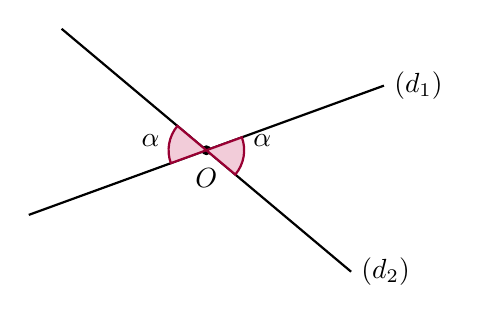
\begin{tikzpicture}[scale=1.2]
    % Les deux droites sécantes définies par des angles précis
    \draw[thick] (200:2) -- (20:2) node[right] {$(d_1)$};
    \draw[thick] (140:2) -- (-40:2) node[right] {$(d_2)$};
    
    \coordinate (O) at (0,0);
    \fill (O) circle (1.5pt) node[below=3pt] {$O$};
    
    % Secteurs angulaires parfaits (gauche et droite)
    \draw[draw=purple!80!black, fill=purple!20, thick] (O) -- (-40:0.4) arc (-40:20:0.4) -- cycle;
    \draw[draw=purple!80!black, fill=purple!20, thick] (O) -- (140:0.4) arc (140:200:0.4) -- cycle;
    
    \node at (10:0.6) {$\alpha$};
    \node at (170:0.6) {$\alpha$};
\end{tikzpicture}
\captionof{figure}{Angles opposés par le sommet (mesures égales).}
\end{center}

\subsubsection{Angles alternes-internes}

\definition{Deux angles sont dits \textbf{alternes-internes} s'ils sont situés de part et d'autre de la sécante, à l'intérieur de la zone délimitée par les deux droites coupées.}

\theorem{Théorème}{Parallélisme et angles alternes-internes}{false}{
Si deux droites parallèles sont coupées par une sécante, alors les angles alternes-internes qu'elles forment ont la même mesure.\\
\textbf{Réciproque :} Si deux droites coupées par une sécante forment deux angles alternes-internes de même mesure, alors ces droites sont parallèles.
}

\noindent{\textbf{Preuve (Propriété directe) :}\\
Soient $(d_1) \parallel (d_2)$ deux droites coupées par une sécante $(\Delta)$ en $A$ et $B$. Soit $I$ le milieu de $[AB]$. La symétrie centrale de centre $I$ transforme $(\Delta)$ en elle-même et échange $A$ et $B$. L'image de $(d_1)$ est une droite parallèle à $(d_1)$ passant par $B$. Par unicité de la parallèle (axiome d'Euclide), cette image est $(d_2)$. La symétrie conservant les angles, l'angle alterne-interne en $A$ est envoyé sur l'angle alterne-interne en $B$. Ils sont donc égaux.
}

\begin{center}
\usetikzlibrary{angles, quotes}
\begin{tikzpicture}[scale=1.2]
    % Définition des points de repère pour tracer les droites
    \coordinate (D1g) at (-1.5, 1.5);
    \coordinate (D1d) at (4, 1.5);
    \coordinate (D2g) at (-1.5, 0);
    \coordinate (D2d) at (4, 0);
    
    % Tracé des droites parallèles
    \draw[thick] (D1g) -- (D1d) node[right] {$(d_1)$};
    \draw[thick] (D2g) -- (D2d) node[right] {$(d_2)$};
    
    % Intersection et tracé de la sécante
    \coordinate (A) at (2, 1.5);
    \coordinate (B) at (0, 0);
    \draw[thick, blue] (-0.5,-0.375) -- (3,2.25) node[above] {$(\Delta)$};
    
    % Points supplémentaires sur la sécante pour orienter les angles
    \coordinate (Top) at (3,2.25);
    \coordinate (Bot) at (-0.5,-0.375);
    
    % Marquage des points d'intersection principaux
    \fill (A) circle (1.5pt) node[above left] {$A$};
    \fill (B) circle (1.5pt) node[below right] {$B$};
    
    % Tracé automatique et parfait des secteurs angulaires alternes-internes
    \pic [draw=orange!80!black, fill=orange!30, thick, angle radius=5mm, "$\alpha$", angle eccentricity=1.4] {angle = D1g--A--B};
    \pic [draw=orange!80!black, fill=orange!30, thick, angle radius=5mm, "$\alpha$", angle eccentricity=1.4] {angle = D2d--B--A};

\end{tikzpicture}
\captionof{figure}{Configuration d'angles alternes-internes égaux.}
\end{center}

\subsubsection{Angles alternes-externes}

\definition{Deux angles sont dits \textbf{alternes-externes} s'ils sont situés de part et d'autre de la sécante, à l'extérieur de la zone délimitée par les deux droites coupées.}

\theorem{Théorème}{Parallélisme et angles alternes-externes}{false}{
Si deux droites parallèles sont coupées par une sécante, alors les angles alternes-externes qu'elles forment ont la même mesure.
}

\noindent{\textbf{Preuve :}\\
Soient $\widehat{1}$ et $\widehat{2}$ deux angles alternes-externes formés par $(d_1) \parallel (d_2)$ et la sécante $(\Delta)$. Soit $\widehat{3}$ l'angle opposé par le sommet à $\widehat{1}$. On a $\widehat{1} = \widehat{3}$. Or, $\widehat{3}$ et $\widehat{2}$ sont en position d'angles alternes-internes, donc $\widehat{3} = \widehat{2}$ puisque $(d_1) \parallel (d_2)$. Par transitivité, on en conclut que $\widehat{1} = \widehat{2}$.
}

\begin{center}
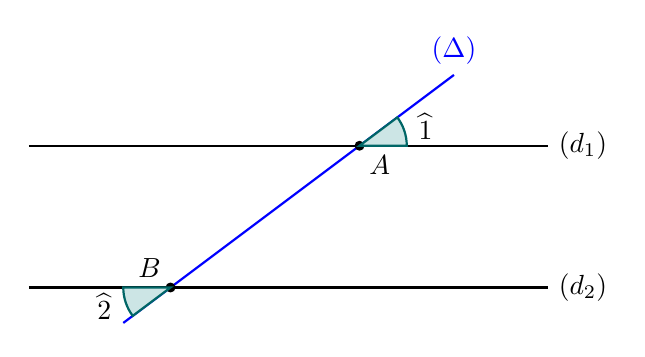
\begin{tikzpicture}[scale=1.2]
    \draw[thick] (-1.5,1.5) -- (4,1.5) node[right] {$(d_1)$};
    \draw[thick] (-1.5,0) -- (4,0) node[right] {$(d_2)$};
    \draw[thick, blue] (-0.5,-0.375) -- (3,2.25) node[above] {$(\Delta)$};
    
    \coordinate (A) at (2,1.5);
    \coordinate (B) at (0,0);
    \fill (A) circle (1.5pt) node[below right] {$A$};
    \fill (B) circle (1.5pt) node[above left] {$B$};
    
    % Secteur en A (externe droit) : centré en A
    \draw[draw=teal!80!black, fill=teal!20, thick, shift={(A)}] (0,0) -- (0:0.5) arc (0:36.87:0.5) -- cycle;
    % Secteur en B (externe gauche) : centré en B (0,0)
    \draw[draw=teal!80!black, fill=teal!20, thick, shift={(B)}] (0,0) -- (180:0.5) arc (180:216.87:0.5) -- cycle;
    
    \node at (2.7,1.7) {$\widehat{1}$};
    \node at (-0.7,-0.2) {$\widehat{2}$};
\end{tikzpicture}
\captionof{figure}{Configuration d'angles alternes-externes égaux.}
\end{center}

\subsubsection{Angles correspondants}

\definition{Deux angles sont dits \textbf{correspondants} s'ils sont situés du même côté de la sécante, l'un à l'intérieur et l'autre à l'extérieur de la zone délimitée par les deux droites.}

\theorem{Théorème}{Parallélisme et angles correspondants}{false}{
Si deux droites parallèles sont coupées par une sécante, alors les angles correspondants qu'elles forment ont la même mesure.
}

\noindent{\textbf{Preuve :}\\
Soient $\widehat{1}$ et $\widehat{2}$ deux angles correspondants. L'angle $\widehat{1}$ possède un angle opposé par le sommet qui se trouve être un angle alterne-interne vis-à-vis de l'angle $\widehat{2}$. Par composition des égalités (les opposés par le sommet étant égaux et les alternes-internes étant égaux sous l'hypothèse de parallélisme), les angles correspondants $\widehat{1}$ et $\widehat{2}$ ont la même mesure.
}

\begin{center}
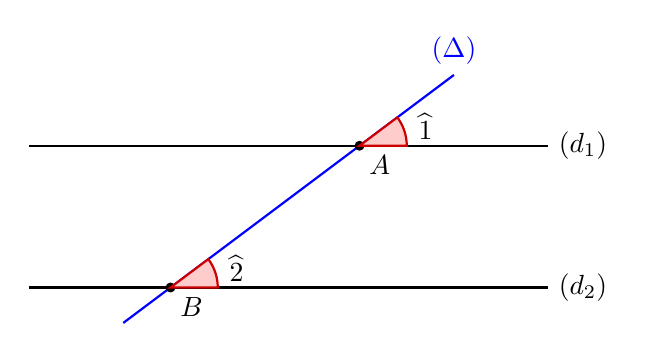
\begin{tikzpicture}[scale=1.2]
    % Droites parallèles et sécante
    \draw[thick] (-1.5,1.5) -- (4,1.5) node[right] {$(d_1)$};
    \draw[thick] (-1.5,0) -- (4,0) node[right] {$(d_2)$};
    \draw[thick, blue] (-0.5,-0.375) -- (3,2.25) node[above] {$(\Delta)$};
    
    % Coordonnées géométriques exactes des intersections
    \coordinate (A) at (2,1.5);
    \coordinate (B) at (0,0);
    \fill (A) circle (1.5pt) node[below right] {$A$};
    \fill (B) circle (1.5pt) node[below right] {$B$};
    
    % Secteur en A (haut droit) : centré en A
    \draw[draw=red!80!black, fill=red!20, thick, shift={(A)}] (0,0) -- (0:0.5) arc (0:36.87:0.5) -- cycle;
    
    % Secteur en B (haut droit) : centré en B (0,0)
    \draw[draw=red!80!black, fill=red!20, thick, shift={(B)}] (0,0) -- (0:0.5) arc (0:36.87:0.5) -- cycle;
    
    % Ajustement fin des étiquettes d'angles
    \node at (2.7,1.7) {$\widehat{1}$};
    \node at (0.7,0.2) {$\widehat{2}$};
\end{tikzpicture}
\captionof{figure}{Configuration d'angles correspondants égaux.}
\end{center}


\section{Propriétés des triangles et droites remarquables}

\subsection{Somme des angles et inégalité triangulaire}

\theorem{Théorème}{Somme des angles}{false}{
Dans un triangle, la somme des mesures des angles est égale à $180^\circ$.
}

\noindent{\textbf{Preuve :}\\
Soit un triangle $ABC$. Traçons la droite $(d)$ parallèle à $(BC)$ passant par $A$. Les angles alternes-internes formés par les droites parallèles $(d)$ et $(BC)$ avec les sécantes $(AB)$ et $(AC)$ montrent que les angles adjacents au sommet $A$ reconstituent un angle plat de $180^\circ$. Ainsi, $\widehat{A} + \widehat{B} + \widehat{C} = 180^\circ$.
}

\theorem{Théorème}{Inégalité triangulaire}{false}{
Dans un triangle $ABC$, la longueur de chaque côté est toujours inférieure à la somme des longueurs des deux autres côtés : $AB \leq AC + CB$. Il y a égalité si et seulement si $C \in [AB]$.
}

\noindent{\textbf{Preuve :}\\
Supposons que $AB > AC + CB$. En traçant le segment $[AC]$ et en prolongeant $[CB]$ au-delà de $B$, on peut trouver un point $D$ tel que $CD = AC$. Par construction, $AD = AC + CD = 2AC$. Cependant, dans le triangle $ABD$, on aurait $AB < AD$, ce qui contredit l'hypothèse. Par conséquent, l'inégalité doit être vérifiée : $AB \leq AC + CB$.
}

\method{Vérifier si un triangle est constructible}{
Pour vérifier si un triangle est constructible, on compare la plus grande longueur à la somme des deux autres. Si la plus grande longueur est strictement inférieure à cette somme, le triangle est constructible.
}

\subsection{Droites remarquables}

\definition{La \textbf{médiatrice} d'un segment est la droite perpendiculaire à ce segment en son milieu. C'est l'ensemble des points équidistants des deux extrémités du segment.}

\remark{Les trois médiatrices d'un triangle sont concourantes en un point qui est le centre du \textbf{cercle circonscrit} au triangle.}

\definition{La \textbf{hauteur} d'un triangle est une droite passant par un sommet et perpendiculaire au côté opposé.}

\definition{La \textbf{bissectrice} d'un angle est la demi-droite qui partage cet angle en deux angles adjacents de même mesure. C'est également l'ensemble des points équidistants des deux côtés de l'angle.}

\remark{Les trois bissectrices d'un triangle sont concourantes en un point qui est le centre du \textbf{cercle inscrit} au triangle.}


\section{Théorèmes fondamentaux de géométrie plane}

\subsection{Théorème de Pythagore}

\theorem{Théorème}{Pythagore (Direct et Réciproque)}{false}{
\begin{itemize}
    \item \textbf{Théorème direct :} Si un triangle $ABC$ est rectangle en $A$, alors le carré de l'hypoténuse est égal à la somme des carrés des deux autres côtés : $BC^2 = AB^2 + AC^2$.
    \item \textbf{Réciproque :} Si dans un triangle $ABC$, on a $BC^2 = AB^2 + AC^2$, alors le triangle est rectangle en $A$.
\end{itemize}
}

\noindent{\textbf{Preuve du théorème direct :}\\
Considérons un triangle $ABC$ rectangle en $A$. Traçons la hauteur issue de $A$, qui coupe $[BC]$ en $H$. 
Les triangles $ABC$ et $HBA$ partagent l'angle $\widehat{B}$ et possèdent chacun un angle droit. Ils sont donc semblables, ce qui donne le rapport : $\frac{BA}{BC} = \frac{BH}{BA}$, d'où $AB^2 = BH \times BC$.
De même, les triangles $ABC$ et $HAC$ sont semblables, ce qui donne : $\frac{CA}{BC} = \frac{CH}{AC}$, d'où $AC^2 = CH \times BC$.
En additionnant membre à membre :
$$AB^2 + AC^2 = (BH + CH) \times BC$$
Comme $H$ appartient au segment $[BC]$, on a $BH + CH = BC$. Ainsi :
$$AB^2 + AC^2 = BC \times BC = BC^2$$
}

\noindent{\textbf{Preuve de la réciproque :}\\
Soit un triangle $ABC$ tel que $BC^2 = AB^2 + AC^2$. 
Construisons un triangle $A'B'C'$ rectangle en $A'$ tel que $A'B' = AB$ et $A'C' = AC$.
Puisque $A'B'C'$ est rectangle en $A'$, on peut lui appliquer le théorème direct de Pythagore :
$$B'C'^2 = A'B'^2 + A'C'^2$$
En substituant les longueurs égales par construction, on obtient :
$$B'C'^2 = AB^2 + AC^2$$
Or, par hypothèse sur le triangle initial, on sait que $AB^2 + AC^2 = BC^2$. On en déduit donc que :
$$B'C'^2 = BC^2 \implies B'C' = BC$$
Les triangles $ABC$ et $A'B'C'$ ont leurs trois côtés respectifs de même longueur ($AB=A'B'$, $AC=A'C'$ et $BC=B'C'$). Ils sont donc égaux (isométriques). 
Par conséquent, tous leurs angles sont égaux deux à deux. Puisque $\widehat{A'} = 90^\circ$, on a nécessairement $\widehat{A} = 90^\circ$. Le triangle $ABC$ est bien rectangle en $A$.
}

\begin{center}
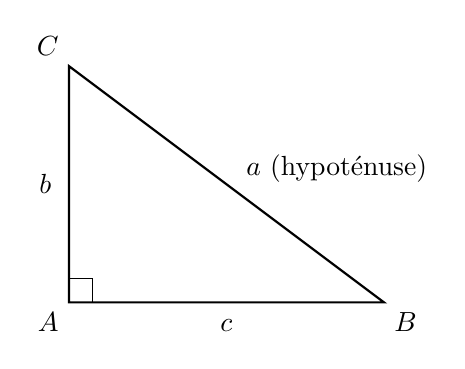
\begin{tikzpicture}[scale=1]
    \draw[thick] (0,0) node[below left] {$A$} -- (4,0) node[below right] {$B$} -- (0,3) node[above left] {$C$} -- cycle;
    \draw (0,0) ++(0.3,0) -- ++(0,0.3) -- ++(-0.3,0);
    \node at (2,-0.3) {$c$};
    \node at (-0.3,1.5) {$b$};
    \node at (3.4,1.7) {$a$ (hypoténuse)};
\end{tikzpicture}
\captionof{figure}{Triangle rectangle : $a^2 = b^2 + c^2$.}
\end{center}

\method{Calculer une longueur avec Pythagore}{
    Si le triangle est rectangle et que l'on connaît la longueur de deux côtés :
    \begin{enumerate}
        \item Écrire l'égalité de Pythagore.
        \item Isoler le côté recherché.
        \item Utiliser la racine carrée ($\sqrt{\, \cdot \,}$) pour trouver la valeur exacte de la longueur.
    \end{enumerate}
}

\attention{La réciproque du théorème de Pythagore sert exclusivement à prouver qu'un triangle \textbf{est rectangle}. Si l'égalité n'est pas vérifiée, on utilise la \textbf{contraposée} du théorème pour conclure que le triangle n'est pas rectangle.}

\example{Soit un triangle $ABC$ tel que $AB=3$ cm, $AC=4$ cm et $BC=5$ cm. On calcule d'une part $BC^2 = 5^2 = 25$, et d'autre part $AB^2 + AC^2 = 3^2 + 4^2 = 9 + 16 = 25$. Comme $BC^2 = AB^2 + AC^2$, d'après la réciproque du théorème de Pythagore, le triangle $ABC$ est rectangle en $A$.}

\subsection{Théorème de Thalès}

\theorem{Théorème}{Thalès (Direct et Réciproque)}{false}{
Soient deux droites $(d)$ et $(d')$ sécantes en un point $A$. Soient $B$ et $M$ deux points de $(d)$ distincts de $A$. Soient $C$ et $N$ deux points de $(d')$ distincts de $A$.
\begin{itemize}
    \item \textbf{Théorème direct :} Si les droites $(BC)$ et $(MN)$ sont parallèles, alors on a l'égalité des rapports : 
    $$\frac{AM}{AB} = \frac{AN}{AC} = \frac{MN}{BC}$$
    \item \textbf{Réciproque :} Si les points $A, M, B$ d'une part et $A, N, C$ d'autre part sont alignés dans le même ordre, et si $\frac{AM}{AB} = \frac{AN}{AC}$, alors les droites $(BC)$ et $(MN)$ sont parallèles.
\end{itemize}
}

\noindent{\textbf{Preuve du théorème direct :}\\
Soient deux droites $(d)$ et $(d')$ sécantes en $A$. Les points $B, M$ sont sur $(d)$ et $C, N$ sur $(d')$, avec $(MN) \parallel (BC)$.
Considérons les triangles $AMN$, $BMN$ et $CMN$.

1. Les triangles $BMN$ et $CMN$ ont une base commune $[MN]$. Comme les droites $(MN)$ et $(BC)$ sont parallèles, la distance entre ces deux droites (qui correspond à la hauteur de ces deux triangles issue de $B$ et $C$) est identique. Leurs aires sont donc égales :
$$\mathcal{A}(BMN) = \mathcal{A}(CMN)$$

2. Exprimons l'aire du triangle $AMN$ de deux manières différentes en traçant les hauteurs du triangle $ABC$ :
\begin{itemize}
    \item En prenant $[AM]$ comme base et la hauteur issue de $N$ notée $h_N$ : $\mathcal{A}(AMN) = \frac{AM \times h_N}{2}$.
    \item De même, l'aire de $BMN$ vaut : $\mathcal{A}(BMN) = \frac{BM \times h_N}{2}$.
\end{itemize}
Le rapport de ces deux aires donne :
$$\frac{\mathcal{A}(AMN)}{\mathcal{A}(BMN)} = \frac{AM}{BM}$$

3. De la même façon, en prenant $[AN]$ comme base et la hauteur issue de $M$ notée $h_M$, on obtient :
$$\frac{\mathcal{A}(AMN)}{\mathcal{A}(CMN)} = \frac{AN}{CN}$$

Puisque $\mathcal{A}(BMN) = \mathcal{A}(CMN)$, les deux rapports d'aires sont égaux, d'où :
$$\frac{AM}{BM} = \frac{AN}{CN} \implies \frac{AM}{AM + BM} = \frac{AN}{AN + CN} \implies \frac{AM}{AB} = \frac{AN}{AC}$$
Le troisième rapport $\frac{MN}{BC}$ s'obtient de manière analogue en traçant une parallèle à $(AB)$ passant par $N$.
}
\vspace{.5cm}

\noindent{\textbf{Preuve du théorème réciproque :}\\
Supposons que les points $A, M, B$ d'une part et $A, N, C$ d'autre part soient alignés dans le même ordre, et que l'on ait :
$$\frac{AM}{AB} = \frac{AN}{AC}$$
Supposons par l'absurde que la droite $(MN)$ ne soit pas parallèle à $(BC)$. Traçons alors la droite parallèle à $(BC)$ passant par $M$. Cette droite coupe le segment $[AC]$ en un point $N'$ distinct de $N$.

Puisque par construction $(MN') \parallel (BC)$, nous pouvons appliquer le théorème de Thalès direct démontré précédemment :
$$\frac{AM}{AB} = \frac{AN'}{AC}$$
Par hypothèse, nous savons également que :
$$\frac{AM}{AB} = \frac{AN}{AC}$$
On en déduit immédiatement l'égalité suivante :
$$\frac{AN'}{AC} = \frac{AN}{AC} \implies AN' = AN$$
Les points $N$ et $N'$ sont situés sur la même demi-droite d'origine $A$ et sont à la même distance de $A$. Ils sont donc confondus ($N = N'$). 
Par conséquent, la droite $(MN)$ est confondue avec la droite $(MN')$, qui est parallèle à $(BC)$. L'hypothèse d'absurde est rejetée : les droites $(BC)$ et $(MN)$ sont bien parallèles.
}

\begin{center}
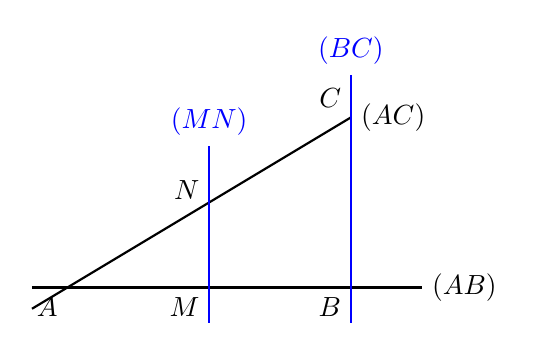
\begin{tikzpicture}[scale=0.9]
    \draw[thick] (-0.5,0) -- (5,0) node[right] {$(AB)$};
    \draw[thick] (-0.5,-0.3) -- (4,2.4) node[right] {$(AC)$};
    \node at (0,0) [below left] {$A$};
    \draw[thick, blue] (2,-0.5) -- (2,2) node[above] {$(MN)$};
    \draw[thick, blue] (4,-0.5) -- (4,3) node[above] {$(BC)$};
    \node at (2,0) [below left] {$M$};
    \node at (4,0) [below left] {$B$};
    \node at (2,1.1) [above left] {$N$};
    \node at (4,2.4) [above left] {$C$};
\end{tikzpicture}
\captionof{figure}{Configuration de Thalès classique (lignes parallèles).}
\end{center}

\toTrain{Entraînez-vous à repérer la configuration en « papillon » de Thalès, où le point d'intersection $A$ se situe entre les deux droites parallèles.}



\subsection{Trigonométrie dans le triangle rectangle}

\definition{Dans un triangle rectangle, pour un des angles aigus $\alpha$ :
$$\cos(\alpha) = \frac{\text{Côté Adjacent}}{\text{Hypoténuse}} \quad ; \quad \sin(\alpha) = \frac{\text{Côté Opposé}}{\text{Hypoténuse}} \quad ; \quad \tan(\alpha) = \frac{\text{Côté Opposé}}{\text{Côté Adjacent}}$$
}

\illustration{Un moyen mnémotechnique classique pour retenir ces formules est le mot \textbf{SOH CAH TOA} (Sinus = Opposé/Hypoténuse, Cosinus = Adjacent/Hypoténuse, Tangente = Opposé/Adjacent).}

\begin{center}
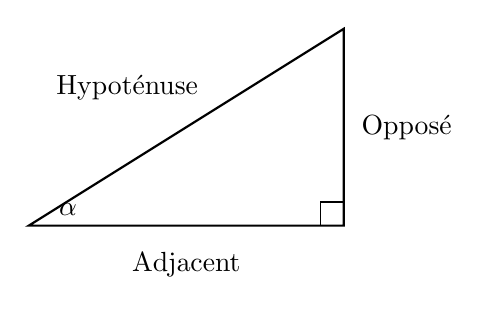
\begin{tikzpicture}[scale=1]
    \draw[thick] (0,0) -- (4,0) -- (4,2.5) -- cycle;
    \draw (4,0) ++(-0.3,0) -- ++(0,0.3) -- ++(0.3,0);
    \node at (0.5,0.2) {$\alpha$};
    \node at (2,-0.5) {Adjacent};
    \node at (4.8,1.25) {Opposé};
    \node at (1.25,1.75) {Hypoténuse};
\end{tikzpicture}
\end{center}

\section{Transformations géométriques du plan}

\subsection{Symétries, translations et rotations}

\definition{\begin{itemize}
    \item \textbf{Symétrie axiale :} Réflexion d'une figure par rapport à un axe (pliage).
    \item \textbf{Symétrie centrale :} Demi-tour d'une figure autour d'un centre $O$. Le symétrique de $M$ par rapport à $O$ est $M'$ tel que $O$ soit le milieu de $[MM']$.
    \item \textbf{Translation :} Glissement d'une figure selon une direction, un sens et une longueur donnée.
    \item \textbf{Rotation :} Pivotement d'une figure autour d'un centre d'un certain angle et dans un sens déterminé (horaire ou anti-horaire).
\end{itemize}
}

\remark{Ces quatre transformations sont des \textbf{isométries} : elles conservent les longueurs, les alignements, les angles et les aires.}

\subsection{Homothéties et similitudes}

\definition{Une \textbf{homothétie} est une transformation qui agrandit ou réduit une figure à partir d'un centre $O$ et d'un rapport $k$ non nul. 
Si $M'$ est l'image de $M$, alors les points $O, M, M'$ sont alignés et $OM' = |k| \times OM$. 
\begin{itemize}
    \item Si $k > 0$, $M$ et $M'$ sont du même côté par rapport à $O$.
    \item Si $k < 0$, $M$ et $M'$ sont de part et d'autre de $O$.
\end{itemize}
}

\begin{center}
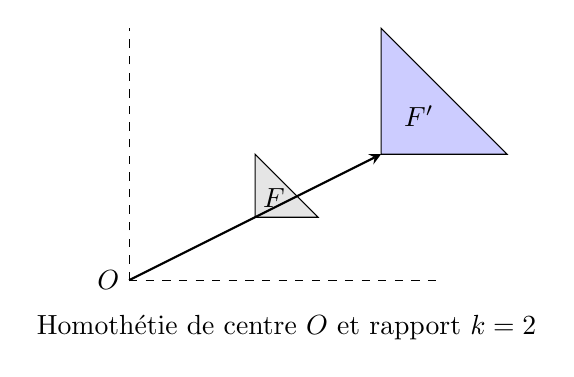
\begin{tikzpicture}[scale=0.8]
    \draw[fill=gray!20] (0,0) -- (1,0) -- (0,1) -- cycle;
    \node at (0.3,0.3) {$F$};
    \draw[dashed] (-2,-1) node[left] {$O$} -- (3,1.5);
    \draw[dashed] (-2,-1) -- (3,-1);
    \draw[dashed] (-2,-1) -- (-2,3);
    \draw[fill=blue!20] (2,1) -- (4,1) -- (2,3) -- cycle;
    \node at (2.6,1.6) {$F'$};
    \draw[->,>=stealth,thick] (-2,-1) -- (2,1);
    \node at (0.5,-1.75) {Homothétie de centre $O$ et rapport $k=2$};
\end{tikzpicture}
\end{center}

\theorem{Propriétés des agrandissements/réductions}{Aires et Volumes}{true}{
Lors d'un agrandissement ou d'une réduction de rapport $k$ ($k>0$) :
\begin{itemize}
    \item Les longueurs sont multipliées par $k$.
    \item Les aires sont multipliées par $k^2$.
    \item Les volumes sont multipliées par $k^3$.
\end{itemize}
}

\section{Géométrie dans l'espace et repérage}

\subsection{Solides de l'espace}

\definition{Le collège introduit l'étude des solides usuels suivants :
\begin{itemize}
    \item \textbf{Pavé droit et Cube  :} Solides à faces rectangulaires ou carrées.
    \item \textbf{Prisme droit et Cylindre :} Solides possédant deux bases superposables et parallèles.
    \item \textbf{Pyramide et Cône :} Solides se terminant par un sommet unique.
    \item \textbf{Sphère et Boule :} La sphère est l'enveloppe extérieure (surface), la boule est le solide plein.
\end{itemize}
}
\begin{center}
\begin{tabular}{cc}
    % --- PREMIÈRE LIGNE ---
    
    % Fig 1 : Pavé droit
    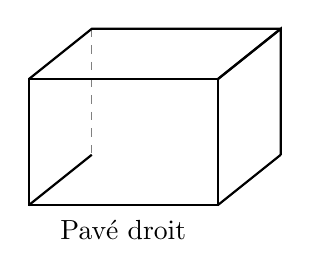
\begin{tikzpicture}[scale=0.8]
        % Faces arrières en pointillés
        \draw[dashed, gray] (0,2) -- (1,2.8) -- (4,2.8);
        \draw[dashed, gray] (1,2.8) -- (1,0.8);
        % Face avant
        \draw[thick] (0,0) rectangle (3,2);
        % Arêtes fuyantes
        \draw[thick] (0,0) -- (1,0.8);
        \draw[thick] (3,0) -- (4,0.8);
        \draw[thick] (3,2) -- (4,2.8);
        % Face supérieure et droite
        \draw[thick] (4,0.8) -- (4,2.8) -- (3,2);
        \draw[thick] (0,2) -- (1,2.8) -- (4,2.8);
        \node at (1.5,-0.4) {Pavé droit};
    \end{tikzpicture}
    &
    % Fig 2 : Cylindre de révolution
    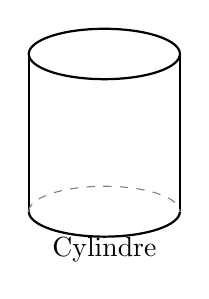
\begin{tikzpicture}[scale=0.8]
        % Base supérieure
        \draw[thick] (0,2.5) ellipse (1.2 and 0.4);
        % Lignes de contour latérales
        \draw[thick] (-1.2,0) -- (-1.2,2.5);
        \draw[thick] (1.2,0) -- (1.2,2.5);
        % Base inférieure (visible devant, pointillée derrière)
        \draw[thick] (-1.2,0) arc (180:360:1.2 and 0.4);
        \draw[dashed, gray] (-1.2,0) arc (180:0:1.2 and 0.4);
        \node at (0,-0.6) {Cylindre};
    \end{tikzpicture}
    \\[2em] % Espace entre les deux lignes
    
    % --- SECONDE LIGNE ---
    
    % Fig 3 : Pyramide à base carrée
    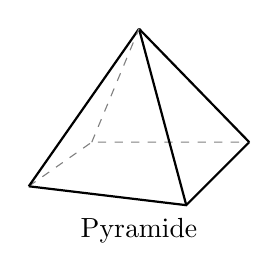
\begin{tikzpicture}[scale=0.8]
        % Base en perspective
        \draw[thick] (0,0) -- (2.5,-0.3) -- (3.5,0.7);
        \draw[dashed, gray] (0,0) -- (1,0.7) -- (3.5,0.7);
        % Sommet
        \coordinate (S) at (1.75,2.5);
        % Arêtes latérales
        \draw[thick] (0,0) -- (S);
        \draw[thick] (2.5,-0.3) -- (S);
        \draw[thick] (3.5,0.7) -- (S);
        \draw[dashed, gray] (1,0.7) -- (S);
        \node at (1.75,-0.7) {Pyramide};
    \end{tikzpicture}
    &
    % Fig 4 : Sphère
    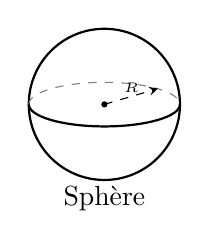
\begin{tikzpicture}[scale=0.8]
        % Contour extérieur
        \draw[thick] (0,0) circle (1.2);
        % Équateur (visible devant, pointillé derrière)
        \draw[thick] (-1.2,0) arc (180:360:1.2 and 0.35);
        \draw[dashed, gray] (-1.2,0) arc (180:0:1.2 and 0.35);
        % Centre et rayon optionnels
        \draw[fill=black] (0,0) circle (0.04);
        \draw[dashed, ->, >=stealth] (0,0) -- (0.85,0.25) node[midway, above=-2pt] {\tiny $R$};
        \node at (0,-1.5) {Sphère};
    \end{tikzpicture}
\end{tabular}
\captionof{figure}{Représentation en perspective cavalière des solides étudiés.}
\end{center}
\method{Calculer un volume}{
\begin{itemize}
    \item \textbf{Prisme / Cylindre :} $\mathcal{V} = \text{Aire de la base} \times \text{hauteur}$
    \item \textbf{Pyramide / Cône :} $\mathcal{V} = \frac{1}{3} \times \text{Aire de la base} \times \text{hauteur}$
    \item \textbf{Boule :} $\mathcal{V} = \frac{4}{3} \times \pi \times \text{rayon}^3$
    \item \textbf{Sphère :} $\mathcal{A} = 4 \times \pi \times \text{rayon}^2$
    \item \textbf{Pavé droit :} $\mathcal{V} = \text{longueur} \times \text{largeur} \times \text{hauteur}$
    \item \textbf{Cube :} $\mathcal{V} = \text{côté}^3$
\end{itemize}
}

\noindent{\textbf{Preuve :}\\
Démontrons rigoureusement ces formules de calcul de volumes et d'aires à l'aide des outils de l'analyse mathématique (calcul intégral).

\begin{itemize}
    \item \textbf{Prisme / Cylindre :} 
    On modélise le solide le long d'un axe vertical $z$, allant de $z = 0$ à $z = h$. Par définition, toutes les sections transversales parallèles à la base ont la même aire constante, notée $\mathcal{A}_{\text{base}}$. En sommant ces sections infiniment fines par intégration, on obtient :
    $$\mathcal{V} = \int_{0}^{h} \mathcal{A}_{\text{base}} \, \mathrm{d}z = \mathcal{A}_{\text{base}} \int_{0}^{h} \mathrm{d}z = \mathcal{A}_{\text{base}} \times h$$
    
    \begin{center}
    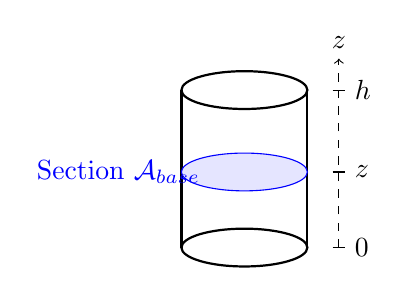
\begin{tikzpicture}[scale=0.8]
        \draw[thick] (0,0) ellipse (1 and 0.3);
        \draw[thick] (0,2.5) ellipse (1 and 0.3);
        \draw[thick] (-1,0) -- (-1,2.5);
        \draw[thick] (1,0) -- (1,2.5);
        \draw[blue, fill=blue!10] (0,1.2) ellipse (1 and 0.3);
        \draw[dashed, ->] (1.5,0) -- (1.5,3) node[above] {$z$};
        \draw (1.4,0) -- (1.6,0) node[right] {$0$};
        \draw (1.4,2.5) -- (1.6,2.5) node[right] {$h$};
        \draw (1.4,1.2) -- (1.6,1.2) node[right] {$z$};
        \node[blue] at (-2,1.2) {Section $\mathcal{A}_{\text{base}}$};
    \end{tikzpicture}
    \end{center}

    \item \textbf{Pyramide / Cône :}
    Considérons un cône ou une pyramide de hauteur $h$ placé le long de l'axe $z$, le sommet pointant à l'origine $z=0$ et la base située à $z=h$. Par Thalès (homothétie), le rapport de réduction linéaire d'une section à l'altitude $z$ est donné par $\frac{z}{h}$. L'aire d'une section variant au carré de ce rapport, on a $\mathcal{A}(z) = \mathcal{A}_{\text{base}} \times \left(\frac{z}{h}\right)^2$. Par intégration :
    $$\mathcal{V} = \int_{0}^{h} \mathcal{A}_{\text{base}} \frac{z^2}{h^2} \, \mathrm{d}z = \frac{\mathcal{A}_{\text{base}}}{h^2} \left[ \frac{z^3}{3} \right]_{0}^{h} = \frac{\mathcal{A}_{\text{base}}}{h^2} \times \frac{h^3}{3} = \frac{1}{3} \times \mathcal{A}_{\text{base}} \times h$$
    
    \begin{center}
    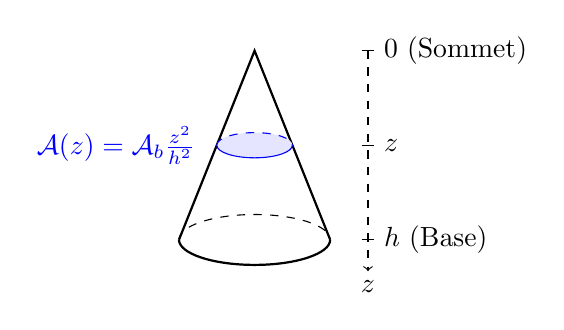
\begin{tikzpicture}[scale=0.8]
        \coordinate (S) at (0,3);
        \draw[thick] (-1.2,0) arc (180:360:1.2 and 0.4);
        \draw[dashed] (-1.2,0) arc (180:0:1.2 and 0.4);
        \draw[thick] (-1.2,0) -- (S) -- (1.2,0);
        \draw[blue, fill=blue!10] (-0.6,1.5) arc (180:360:0.6 and 0.2);
        \draw[blue, dashed, fill=blue!10] (-0.6,1.5) arc (180:0:0.6 and 0.2);
        \draw[dashed, ->] (1.8,3) -- (1.8,-0.5) node[below] {$z$};
        \draw (1.7,3) -- (1.9,3) node[right] {$0$ (Sommet)};
        \draw (1.7,1.5) -- (1.9,1.5) node[right] {$z$};
        \draw (1.7,0) -- (1.9,0) node[right] {$h$ (Base)};
        \node[blue] at (-2.2,1.5) {$\mathcal{A}(z) = \mathcal{A}_b \frac{z^2}{h^2}$};
    \end{tikzpicture}
    \end{center}

    \item \textbf{Boule :}
    Une boule de rayon $R$ peut être modélisée comme un solide de révolution obtenu en faisant tourner le demi-cercle d'équation $y = \sqrt{R^2 - x^2}$ autour de l'axe des abscisses pour $x \in [-R, R]$. Chaque section perpendiculaire à l'axe $x$ à la position $x$ est un disque de rayon $y$, donc d'aire $\pi y^2 = \pi(R^2 - x^2)$. Le volume s'obtient en intégrant ces aires de disques :
    $$\mathcal{V} = \int_{-R}^{R} \pi (R^2 - x^2) \, \mathrm{d}x = \pi \left[ R^2x - \frac{x^3}{3} \right]_{-R}^{R} = \pi \left( \left(R^3 - \frac{R^3}{3}\right) - \left(-R^3 + \frac{R^3}{3}\right) \right) = \frac{4}{3}\pi R^3$$
    
    \begin{center}
    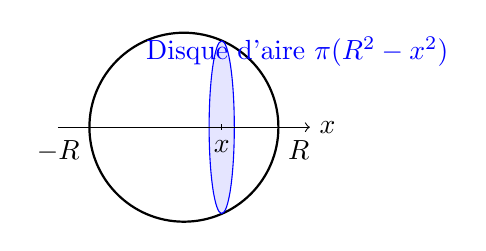
\begin{tikzpicture}[scale=0.8]
        \draw[thick] (0,0) circle (1.5);
        \draw[dashed] (-1.5,0) -- (1.5,0);
        \draw[blue, fill=blue!10] (0.6,0) ellipse (0.2 and 1.37);
        \draw[->] (-2,0) -- (2,0) node[right] {$x$};
        \draw (0.6,0.05) -- (0.6,-0.05) node[below] {$x$};
        \draw (-1.5,0.05) -- (-1.5,-0.05) node[below left] {$-R$};
        \draw (1.5,0.05) -- (1.5,-0.05) node[below right] {$R$};
        \node[blue] at (1.8,1.2) {Disque d'aire $\pi(R^2-x^2)$};
    \end{tikzpicture}
    \end{center}

    \item \textbf{Sphère :}
    L'aire de la surface d'une sphère correspond à la variation de son volume lorsqu'on augmente infinitésimalement le rayon d'une épaisseur $\mathrm{d}r$. Géométriquement, une coquille sphérique d'épaisseur $\mathrm{d}r$ a un volume égal à $\mathcal{A}_{\text{sphère}} \times \mathrm{d}r$. Par le théorème fondamental de l'analyse, l'aire est la dérivée du volume par rapport au rayon $r$ :
    $$\mathcal{A} = \frac{\mathrm{d}\mathcal{V}}{\mathrm{d}r} = \frac{\mathrm{d}}{\mathrm{d}r}\left(\frac{4}{3}\pi r^3\right) = \frac{4}{3}\pi \times 3r^2 = 4\pi r^2$$
    
    \begin{center}
    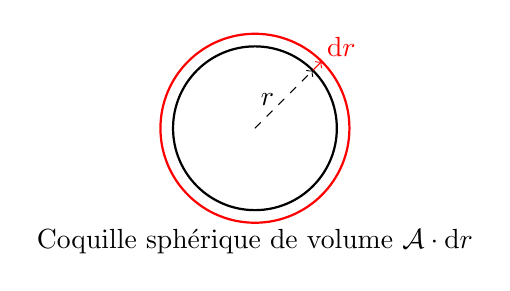
\begin{tikzpicture}[scale=0.8]
        \draw[thick] (0,0) circle (1.3);
        \draw[thick, red] (0,0) circle (1.5);
        \draw[dashed, ->] (0,0) -- (0.92,0.92) node[midway, left] {$r$};
        \draw[red, ->] (0.92,0.92) -- (1.06,1.06) node[midway, above right] {$\mathrm{d}r$};
        \node at (0,-1.8) {Coquille sphérique de volume $\mathcal{A} \cdot \mathrm{d}r$};
    \end{tikzpicture}
    \end{center}

    \item \textbf{Pavé droit :}
    En plaçant le pavé droit dans un repère cartésien orthogonal sur l'intervalle $[0, L] \times [0, \ell] \times [0, h]$, le volume est modélisé par l'intégrale triple de l'élément de volume cartésien $\mathrm{d}\mathcal{V} = \mathrm{d}x\,\mathrm{d}y\,\mathrm{d}z$ :
    $$\mathcal{V} = \int_{0}^{L} \mathrm{d}x \times \int_{0}^{\ell} \mathrm{d}y \times \int_{0}^{h} \mathrm{d}z = [x]_0^L \times [y]_0^\ell \times [z]_0^h = L \times \ell \times h$$
    
    \begin{center}
    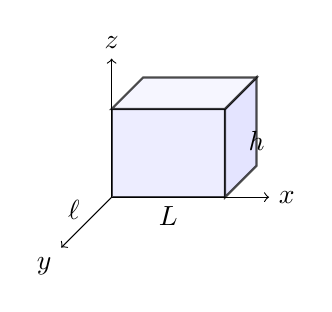
\begin{tikzpicture}[scale=0.8]
        \draw[->] (0,0) -- (2.5,0) node[right] {$x$};
        \draw[->] (0,0) -- (0,2.2) node[above] {$z$};
        \draw[->] (0,0) -- (-0.8,-0.8) node[below left] {$y$};
        \draw[thick, fill=blue!10, opacity=0.7] (0,0) rectangle (1.8,1.4);
        \draw[thick, fill=blue!15, opacity=0.7] (1.8,0) -- (2.3,0.5) -- (2.3,1.9) -- (1.8,1.4) -- cycle;
        \draw[thick, fill=blue!5, opacity=0.7] (0,1.4) -- (0.5,1.9) -- (2.3,1.9) -- (1.8,1.4) -- cycle;
        \node at (0.9,-0.3) {$L$};
        \node at (2.3,0.9) {$h$};
        \node at (-0.6,-0.2) {$\ell$};
    \end{tikzpicture}
    \end{center}

    \item \textbf{Cube :}
    Le cube est un pavé droit uniforme où les trois dimensions de l'espace possèdent une longueur identique égale à $c$. Par application de la formule précédente où $L = \ell = h = c$ :
    $$\mathcal{V} = c \times c \times c = c^3$$
    
    \begin{center}
    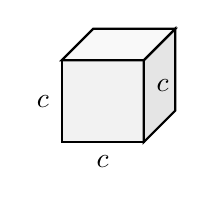
\begin{tikzpicture}[scale=0.8]
        \draw[thick, fill=gray!10] (0,0) rectangle (1.3,1.3);
        \draw[thick, fill=gray!20] (1.3,0) -- (1.8,0.5) -- (1.8,1.8) -- (1.3,1.3) -- cycle;
        \draw[thick, fill=gray!5] (0,1.3) -- (0.5,1.8) -- (1.8,1.8) -- (1.3,1.3) -- cycle;
        \node at (0.65,-0.3) {$c$};
        \node at (1.6,0.9) {$c$};
        \node at (-0.3,0.65) {$c$};
    \end{tikzpicture}
    \end{center}
\end{itemize}
}

\subsection{Repérage}

\vocabulary{On appelle \textbf{repère} un ensemble de points de référence permettant de localiser un point dans le plan ou dans l'espace.}

\definition{
\begin{itemize}
    \item \textbf{Dans le plan :} Un point est repéré par un couple de coordonnées $(x ; y)$ : son \textbf{abscisse} (axe horizontal) et son \textbf{ordonnée} (axe vertical) dans un repère orthogonal.
    \item \textbf{Dans l'espace :} Dans un pavé droit, un point est localisé par un triplet $(x ; y ; z)$ représentant respectivement l'abscisse, l'ordonnée et l'\textbf{altitude} (ou la côte).
    \item \textbf{Sur une sphère :} Le repérage se fait à l'aide de coordonnées géographiques : la \textbf{latitude} (par rapport à l'Équateur) et la \textbf{longitude} (par rapport au méridien de Greenwich).
\end{itemize}
}

\attention{Attention à l'ordre d'écriture des coordonnées : l'abscisse se lit et s'écrit toujours avant l'ordonnée, de même pour la latitude qui précède généralement la longitude.}

\newpage
\tableofcontents

\end{document}